\documentclass{article}

\usepackage{color}
\usepackage{graphicx}
\usepackage{amsmath}
\usepackage{bm}
\usepackage{enumerate}
\usepackage{booktabs}
\usepackage{cite}
\usepackage{geometry}
\usepackage{url}
\usepackage{float}
\usepackage{indentfirst}
\usepackage{ulem}
\usepackage{multirow}
\usepackage{pdfpages}

\begin{document}

\vspace*{0.25cm}

\noindent\hrulefill

\thispagestyle{empty}

\begin{center}
    \begin{large}
        \sc{UM--SJTU Joint Institute \vspace{0.3em} \\ Introduction to Circuits \\(Ve215)}
    \end{large}

    \hrulefill

    \vspace*{5cm}
    \begin{Large}
        \sc{{Laboratory Report}}
    \end{Large}

    \vspace{2em}

    \begin{large}
        \sc{{Lab 5
                    \vspace{0.5em}

                    Filter Lab}}
    \end{large}
\end{center}
\vfill

\begin{table}[h!]
    \flushleft
    \begin{tabular}{ll}
        Name: Kang Jiaming \hspace*{2em} &
        ID: 518021911220\hspace*{2em}     \\

        \\

        Date:  13 Nov. 2019
    \end{tabular}
\end{table}

\hfill
\newpage

\section{Goals}
\begin{enumerate}
    \item Learn about four types of filters – Low-Pass, High-Pass, Band-Pass, and Band-reject.
    \item Learn about transfer functions.
    \item Predict the theoretical result and make comparison with lab data.
\end{enumerate}

\section{Introduction\label{intro}}

\subsection{Filter}
Filters are everywhere in our lives. The circuits built to operate on signals usually apply filters. For example, telephone lines pass the sounds at frequencies between about 100 Hz and 3 kHz and practically blocks all other frequencies.

\subsection{Transfer function}
Mathematically, the transfer function is used to analyze what the circuit did to the signal:
$$\text{Transfer function} = \frac{\text{Output signal}}{\text{Input signal}}$$

This function can also be expressed as
$$H(\omega) = \frac{V_{out}(\omega)}{V_{in}(\omega)}$$

The magnitude of the transfer function is called "voltage gain", often measured as the ratio of the peak-to-peak (ppk) voltages
$$|H(\omega)|=\bigg|\frac{V_{out}(\omega)}{V_{in}(\omega)}\bigg| = \frac{V_{out,ppk}(\omega)}{V_{in,ppk}(\omega)}$$

It is convenient to express and plot the magnitude of the transfer function on the logarithmic scale decibels:
$$|H(\omega)|_{dB} = 20\log_{10}\bigg(\frac{V_{out,ppk}(\omega)}{V_{in,ppk}(\omega)}\bigg)$$

Since both ppk voltages are always positive, the transfer function magnitude is positive and thus can always be converted to decibels. The use of decibels allows us to review data over a broad range.

\subsection{Types of filters}
\begin{figure}[H]\centering
    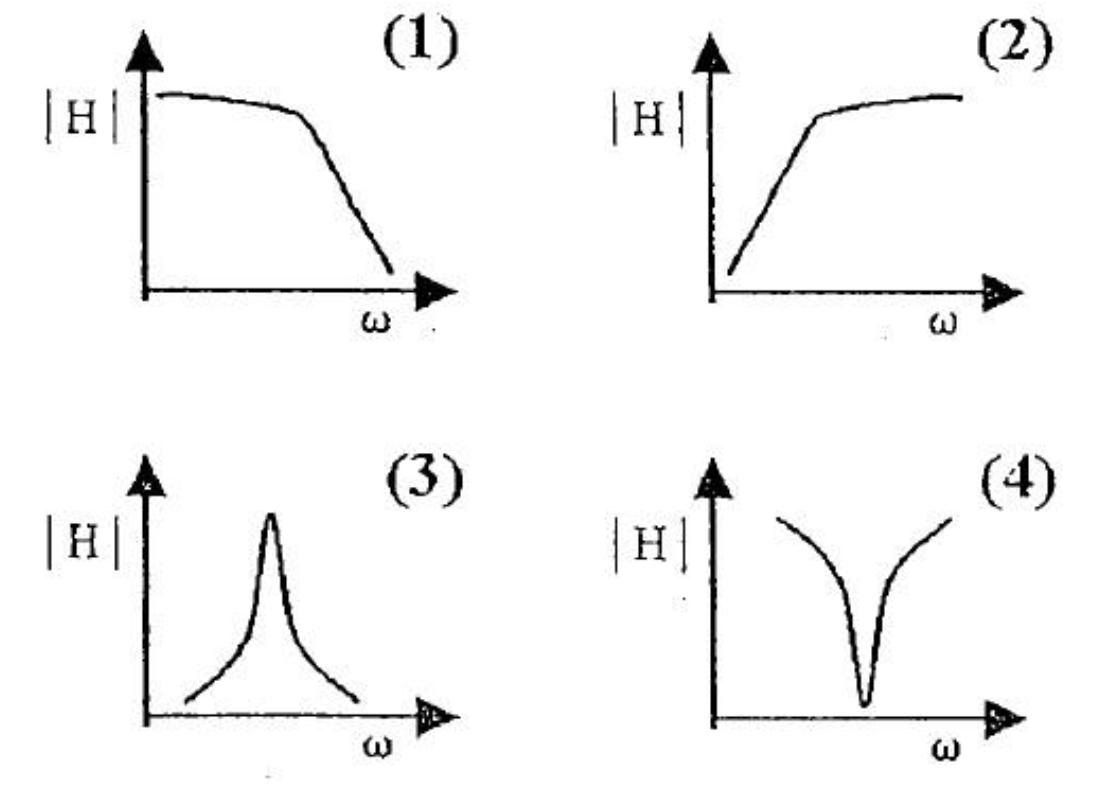
\includegraphics[scale=0.6]{type.png}
    \caption{(1) Low-Pass; (2) High-Pass; (3) Band-Pass; (4) Band-reject (band-stop or north);}
\end{figure}

\begin{figure}[H]\centering
    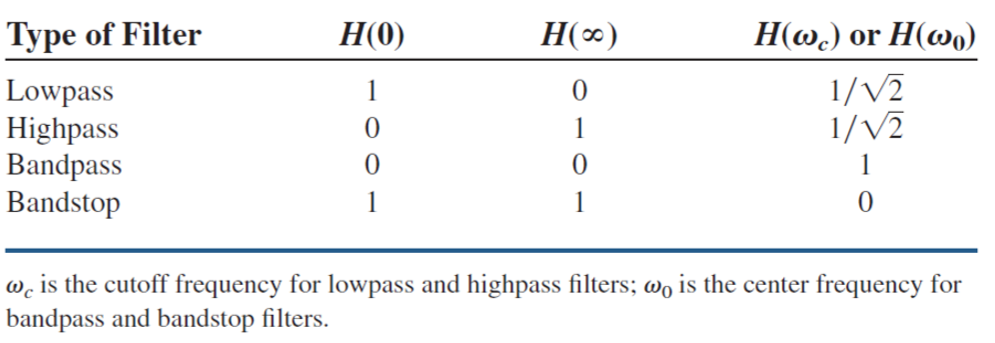
\includegraphics[scale=0.7]{summary.png}
    \caption{Summary of the characteristics of ideal filters.}
\end{figure}

Filter circuits, which you are going to build in this lab, contain resistors, capacitors, and inductors. They are all passive filters.

\subsubsection{High-Pass filter}
The high-pass filter we are going to build uses a capacitor and a resistor.
\begin{figure}[H]\centering
    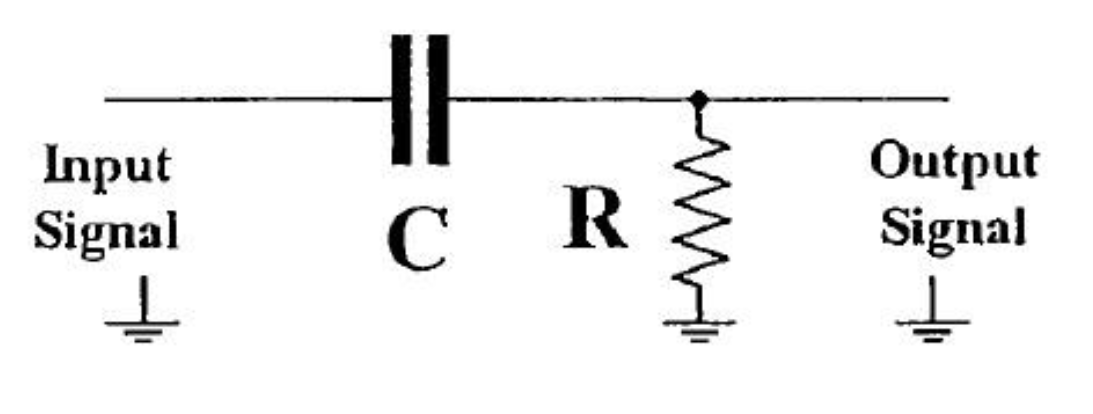
\includegraphics[scale=0.6]{highpass.png}
    \caption{High-Pass filter.}
\end{figure}

For the high-pass filter,
$$H(\omega) = \frac{V_{out}(\omega)}{V_{in}(\omega)} = \frac{R}{R+\frac{1}{j\omega C}} = \frac{j\omega RC}{1+j\omega RC}.$$
Note that $H(0) = 0, H(\infty) = 1$. Hence, it would only let high frequency pass.

\subsubsection{Low-Pass filter}
The low-pass filter we are going to build uses a capacitor and a resistor.
\begin{figure}[H]\centering
    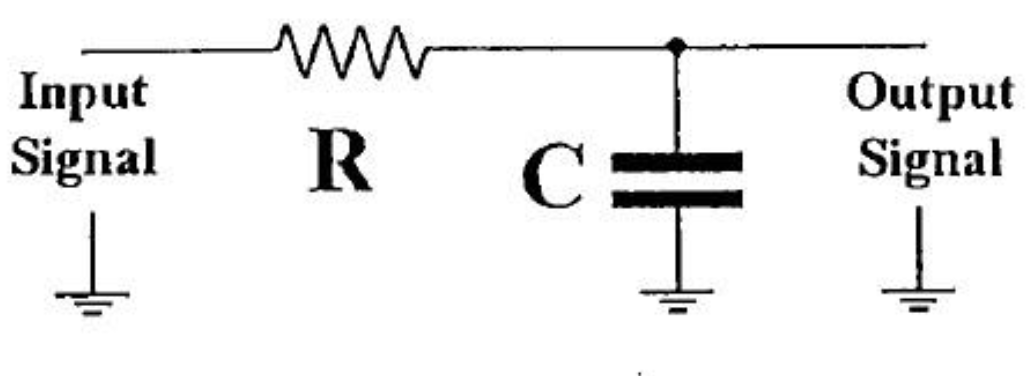
\includegraphics[scale=0.6]{lowpass.png}
    \caption{Low-Pass filter.}
\end{figure}

For the low-pass filter,
$$H(\omega) = \frac{V_{out}(\omega)}{V_{in}(\omega)} = \frac{\frac{1}{j\omega C}}{R+\frac{1}{j\omega C}} = \frac{1}{1+j\omega RC}.$$
Note that $H(0) = 1, H(\infty) = 0$. It would only let low frequency pass.

\subsubsection{Band-Pass filter}
The band-pass filter we are going to build uses a capacitor, an inductor and a resistor.
\begin{figure}[H]\centering
    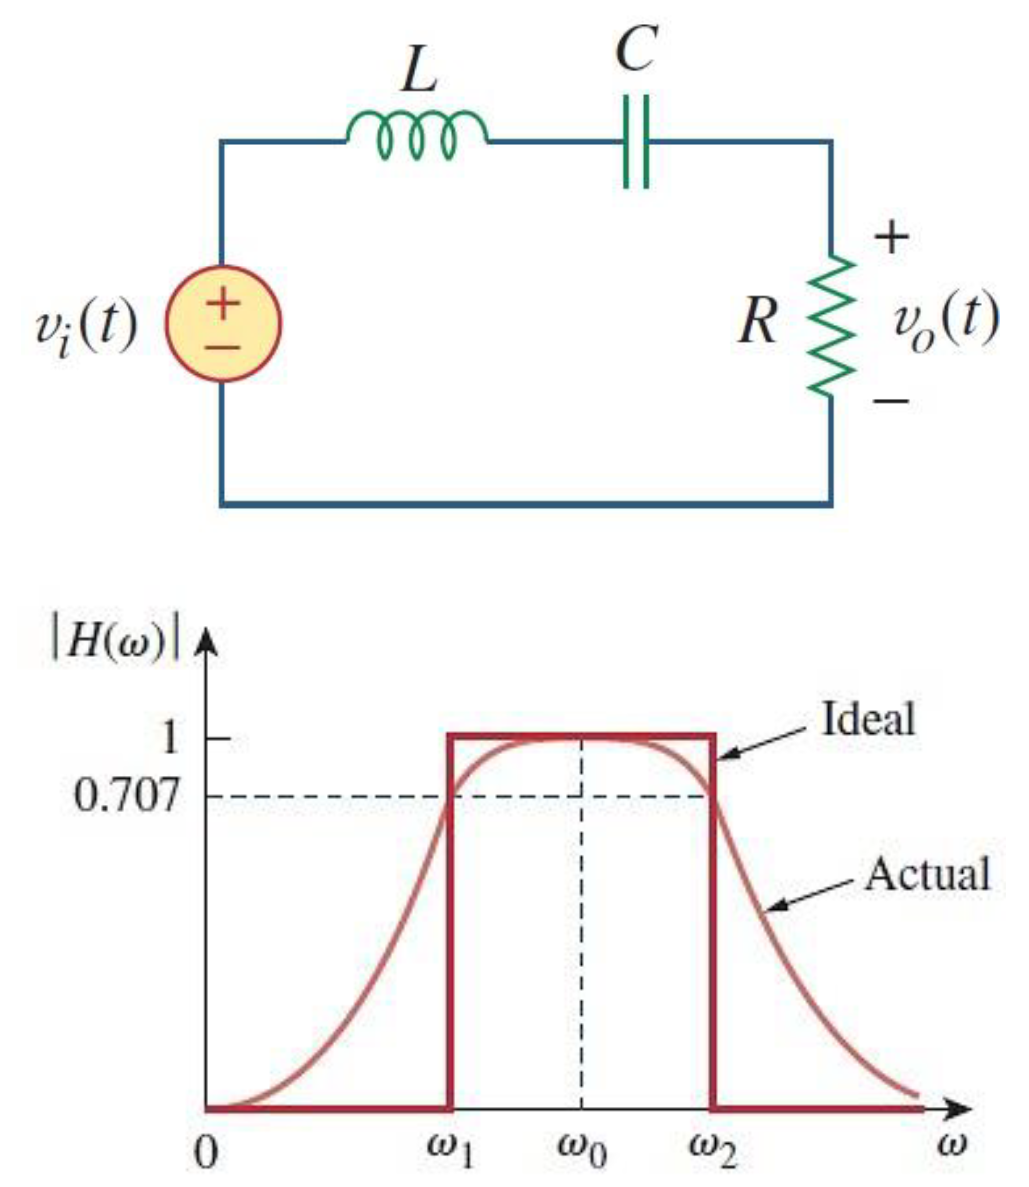
\includegraphics[scale=0.5]{bandpass.png}
    \caption{Band-Pass filter.}
\end{figure}

For the band-pass filter,
$$H(\omega) = \frac{V_{out}(\omega)}{V_{in}(\omega)} = \frac{R}{R+j(\omega L-\frac{1}{\omega C})}.$$
Note that $H(0) = 0, H(\infty) = 0.$ The band-pass filter passes a band of frequencies centered on the center frequency $\omega_0$, which is given by $\omega_0 = 1/\sqrt{LC}$.

\subsubsection{Band-Stop filter}
The band-stop filter we are going to build uses a capacitor, an inductor and a resistor.
\begin{figure}[H]\centering
    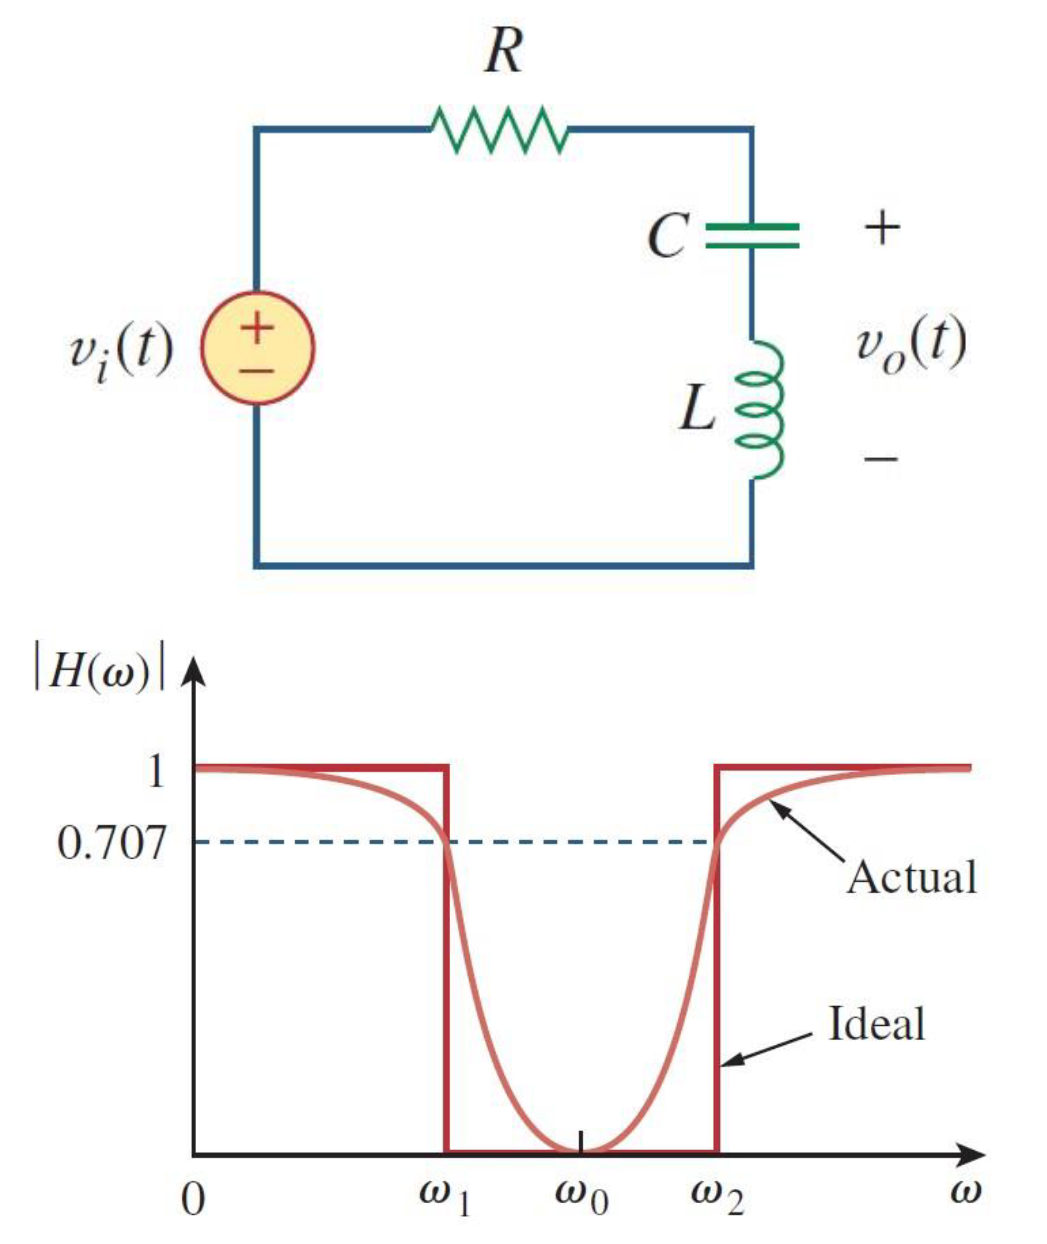
\includegraphics[scale=0.6]{bandstop.png}
    \caption{Band-Stop filter}
\end{figure}

For the band-stop filter,
$$H(\omega) = \frac{V_{out}(\omega)}{V_{in}(\omega)} = \frac{j(\omega L-\frac{1}{\omega C})}{R+j(\omega L-\frac{1}{\omega C})}.$$
Note that $H(0) = 0, H(\infty) = 0.$ The band-stop filter rejects a band of frequencies centered on the center frequency $\omega_0$, which is given by $\omega_0 = 1/\sqrt{LC}$.

\section{Procedures}
\begin{enumerate}
    \item Construct the circuit for each type of filter with resistor 1000 $\Omega$, capacitor 0.1 $\mu$F, inductor 1 mH.
    \item Set the input signal in the function generator to be sine wave with amplitude of 5 Vppk and change the frequency accordingly.
    \item Use the oscilloscope to detect the amplitudes of the input and output signals. Records them respectively in the first two column in the tables.
    \item Calcultate with the experimental data for the transfer function magnitude and transfer function magnitude in dB.
\end{enumerate}



\section{Results}
In this section, for each type of filter, the value of transfer function magnitude and transfer function magnitude in dB are calculated from the corresponding experimental data using the definition formula of transfer function. All the results are presented below.

\subsection{Low-pass Filter}
The data for the low-pass filter are shown in Table \ref{TableLowpass}.

\begin{table}[H]\centering
    \begin{tabular}{ccccccccc}
        \toprule
        Frequency & Input [$V_{ppk}$] & Output [$V_{ppk}$] & $|H|$  & $|H|_{theory}$ & $\epsilon_H$ & dB       & dB$_{theory}$ & $\epsilon_{\text{dB}}$ \\
        \midrule
        1 MHz     & 5.16              & 0.0156 & 0.00302 & 0.0016         & 88.95$\%$    & -50.391 & -55.8048      & -9.88 $\%$             \\
        100 kHz   & 5.12              & 0.110  & 0.021   & 0.0162         & 31.00$\%$    & -33.358 & -35.8070      & -6.57 $\%$             \\
        50 kHz    & 5.08              & 0.232  & 0.0457  & 0.0324         & 39.24$\%$    & -26.808 & -29.7898      & -9.69 $\%$             \\
        10 kHz    & 5.08              & 1.090  & 0.215   & 0.1600         & 32.53$\%$    & -13.369 & -15.9184      & -15.47$\%$              \\
        5 kHz     & 5.08              & 1.820  & 0.358   & 0.3083         & 14.90$\%$    & -8.916  & -10.2191      & -11.92$\%$              \\
        1 kHz     & 5.20              & 4.640  & 0.892   & 0.8510         & 4.50 $\%$    & -0.990  & -1.4010       & -27.86$\%$               \\
        500 Hz    & 5.20              & 5.120  & 0.985   & 0.9556         & 2.93 $\%$    & -0.135  & -0.3948       & -65.06$\%$              \\
        \bottomrule
    \end{tabular}
    \caption{Data for the low-pass filter.}\label{TableLowpass}
\end{table}

\subsection{High-pass Filter}
The data for the high-pass filter are shown in Table \ref{TableHighpass}.

\begin{table}[H]\centering
    \begin{tabular}{ccccccccc}
        \toprule
        Frequency & Input [$V_{ppk}$] & Output [$V_{ppk}$] & $|H|$  & $|H|_{theory}$ & $\epsilon_H$ & dB       & dB$_{theory}$ & $\epsilon_{\text{dB}}$ \\
        \midrule
        1 MHz     & 5.16              & 4.64               & 0.899 & 1.0000         & -10.08$\%$     & -0.923  & 0.000       & /                 \\
        100 kHz   & 5.12              & 4.60               & 0.898 & 0.9999         & -10.15$\%$     & -0.930  & -0.001      & 106993$\%$             \\
        50 kHz    & 5.08              & 4.56               & 0.898 & 0.9995         & -10.19$\%$     & -0.938  & -0.004      & 21492$\%$               \\
        10 kHz    & 5.08              & 4.40               & 0.866 & 0.9871         & -12.23$\%$     & -1.248  & -0.115      & 981.49$\%$              \\
        5 kHz     & 5.12              & 4.16               & 0.813 & 0.9513         & -14.48$\%$     & -1.804  & -0.445      & 305.64$\%$              \\
        1 kHz     & 5.24              & 1.98               & 0.378 & 0.5251         & -27.39$\%$     & -8.453  & -5.673      & 49.00$\%$               \\
        500 Hz    & 5.28              & 1.19               & 0.225 & 0.2948         & -22.68$\%$     & -12.942 & -10.707     & 20.87$\%$              \\
        100 Hz    & 5.28              & 0.258              & 0.049 & 0.0616         & -19.63$\%$     & -26.220 & -24.322     & 7.81$\%$             \\
        \bottomrule
    \end{tabular}
    \caption{Data for the high-pass filter.}\label{TableHighpass}
\end{table}

\subsection{Band-pass Filter}
The data for the band-pass filter are shown in Table \ref{TableBandpass}.

\begin{table}[H]\centering
    \begin{tabular}{ccccccccc}
        \toprule
        Frequency & Input [$V_{ppk}$] & Output [$V_{ppk}$] & $|H|$  & $|H|_{theory}$ & $\epsilon_H$ & dB       & dB$_{theory}$ & $\epsilon_{\text{dB}}$ \\
        \midrule
        1 MHz     & 5.40              & 0.400  & 0.074 & 0.1545         & -51.46$\%$   & -22.607 & -16.329     & 38.45$\%$              \\
        500 kHz   & 5.40              & 1.48   & 0.274 & 0.2986         & -7.19$\%$    & -11.243 & -10.595     & 6.12$\%$               \\
        100 kHz   & 5.16              & 4.08   & 0.791 & 0.8485         & -6.49$\%$    & -2.040  & -1.457      & 40.03$\%$              \\
        50 kHz    & 5.08              & 4.40   & 0.866 & 0.9611         & -9.80$\%$    & -1.248  & -0.353      & 254$\%$               \\
        10 kHz    & 5.08              & 4.44   & 0.874 & 0.9952         & -12.17$\%$   & -1.170  & -0.043      & 2641$\%$                \\
        1 kHz     & 5.24              & 1.98   & 0.378 & 0.5266         & -27.60$\%$   & -8.453  & -5.648      & 49.66$\%$              \\
        500 Hz    & 5.24              & 1.10   & 0.210 & 0.2951         & -28.06$\%$   & -13.559 & -10.698     & 26.74$\%$              \\
        \bottomrule
    \end{tabular}
    \caption{Data for the band-pass filter.}\label{TableBandpass}
\end{table}

\subsection{Band-reject Filter}
The data for the band-reject filter are shown in Table \ref{TableBandreject}.

\begin{table}[H]\centering
    \begin{tabular}{ccccccccc}
        \toprule
        Frequency & Input [$V_{ppk}$] & Output [$V_{ppk}$] & $|H|$  & $|H|_{theory}$ & $\epsilon_H$ & dB       & dB$_{theory}$ & $\epsilon_{\text{dB}}$ \\
        \midrule
        1 MHz     & 5.28              & 3.52  & 0.667 & 0.9880         & -32.54$\%$    & -3.522 & -0.1049       & 3345.20$\%$              \\
        500 kHz   & 5.40              & 4.72  & 0.874 & 0.9544         & -8.51 $\%$    & -1.169 & -0.4056       & 194.99$\%$              \\
        300 kHz   & 5.40              & 4.68  & 0.867 & 0.8863         & -2.47 $\%$    & -1.243 & -1.0481       & 21.16$\%$             \\
        200 kHz   & 5.36              & 4.04  & 0.754 & 0.7860         & -4.55 $\%$    & -2.456 & -2.0911       & 19.74$\%$               \\
        100 kHz   & 5.16              & 2.46  & 0.477 & 0.5292         & -10.71$\%$    & -6.434 & -5.5282       & 18.04$\%$              \\
        50 kHz    & 5.08              & 1.20  & 0.236 & 0.2763         & -15.48$\%$    & -12.534& -11.1721      & 13.20$\%$              \\
        10 kHz    & 5.08              & 0.744 & 0.146 & 0.0976         & 48.24$\%$     & -16.686& -20.2092      & -17.01$\%$             \\
        5 kHz     & 5.08              & 1.68  & 0.331 & 0.2804         & 16.61$\%$     & -9.611 & -10.38        & -12.19$\%$              \\
        1 kHz     & 5.24              & 4.20  & 0.802 & 0.8501         & -6.03$\%$     & -1.922 & -1.4105       & 39.15$\%$               \\
        500 Hz    & 5.24              & 4.60  & 0.878 & 0.9555         & -8.22$\%$     & -1.131 & -0.3956       & 192.90$\%$              \\
        \bottomrule
    \end{tabular}
    \caption{Data for the band-reject filter.}\label{TableBandreject}
\end{table}

\section{Conclusions and discussion}

As can be seen from Table \ref{TableLowpass}$\sim$\ref{TableBandreject}, the experimental data basically conforms to the theoretical value. Therefore the trend of the change of value of transfer function with regard to frequency shown in Figure 1 for all the 4 types of filters is verified.

However, it should be noticed that some of our experimental data are not desirable. Some are of a relatively large error. This may because the measurement of the oscillator is not stable and the resolution and precision of it is not that sufficient. Also, since the measurement result displayed on the oscilloscope is not stable, all the readings are subjectively chosen by us. This may result in some uncertainty. Despite such discrepancy, our experimental results are acceptable in a certain range of uncertainty.

For improvement, apparatus with higher precision and resolution can be utilized.

To sum up, in this lab, we learn and construct four typical types of filters. Besides, the filtering property for each type is explored. Particularly, we examine the relationship between the transfer function and the frequency for each filter. The result of our experiment indicates conforms to the theoretical fact in an acceptable range.

\section{References}
\noindent [1] UM-SJTU Joint Institute VE215 "Filter Lab" lab manual.

\section{Appendix}

Please find the data sheet at the end of the report.

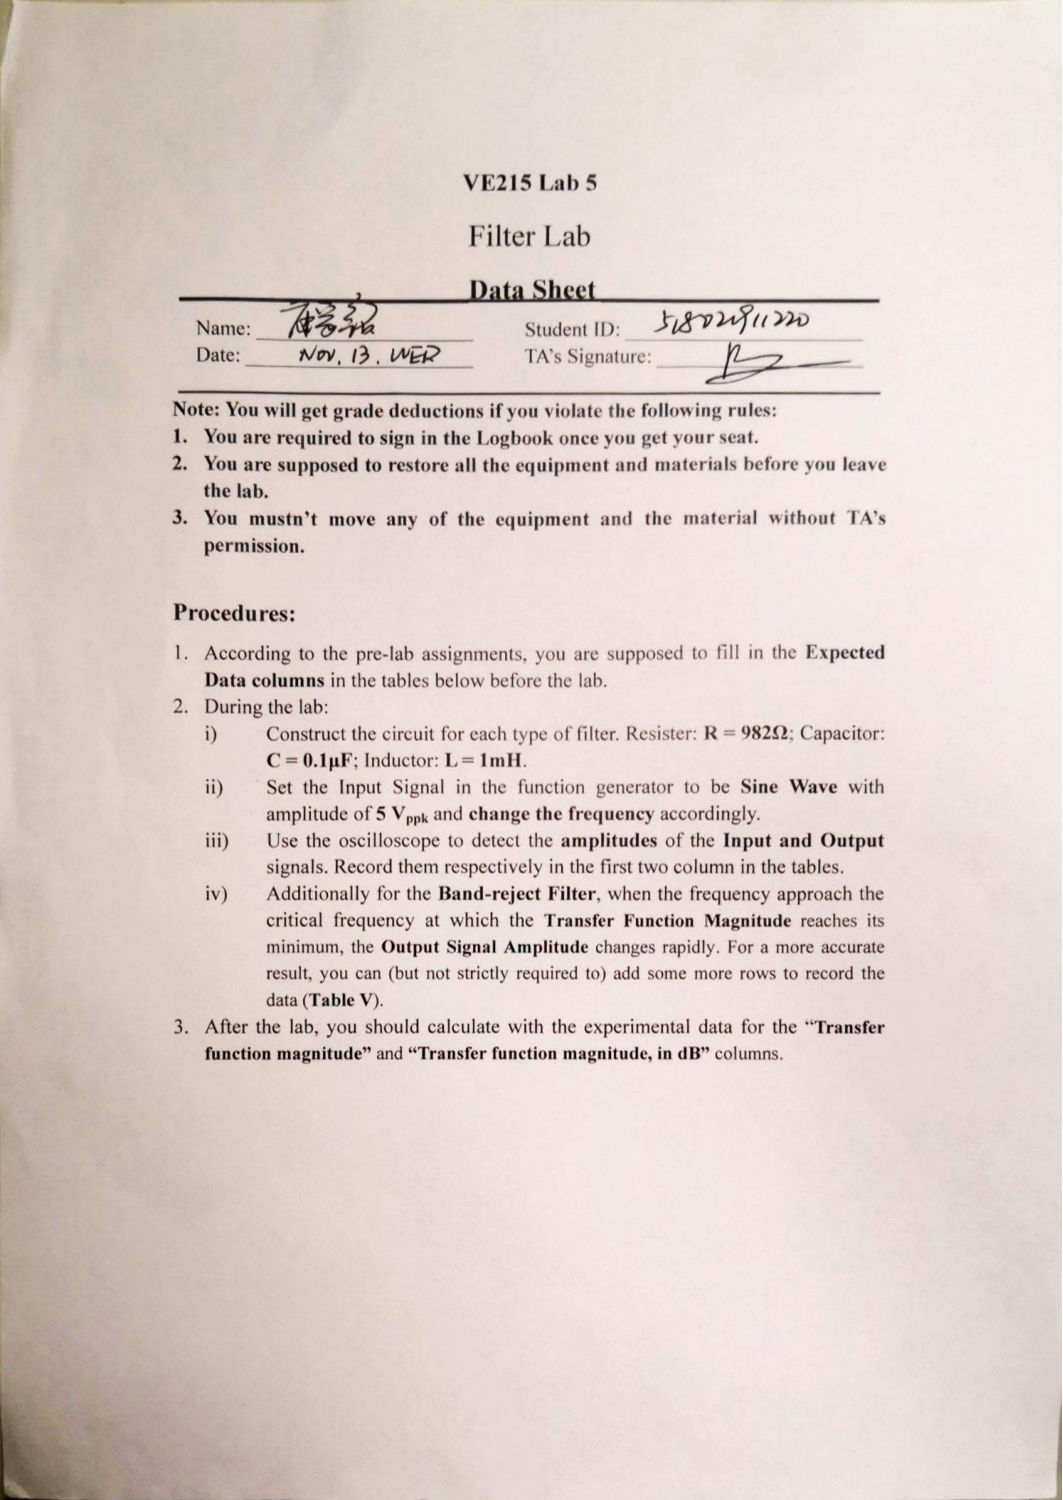
\includepdf[pages=-]{lab5datasheet.pdf}

\end{document}
